\subsection{Számítógépes kódok}

%79
\begin{frame}
  Számítógépes programok írásához kapcsolódó elemek:
  \begin{columns}[c]
    \column{0.5\textwidth}
      \begin{description}[m]
        \item[\texttt{<kbd>}] (keyboard) \hfill \\ Felhasználói adatbevitelre, pl. gépelésre, szóbeli parancsra van szükség.
        \item[\texttt{<samp>}] (sample) \hfill \\ Egy program lehetséges kimenetét mutatja.
        \item[\texttt{<code>}] \hfill \\ Programkód jelölésére. Nem őrzi meg a tördelést $\to$ \texttt{<pre>}
        \item[\texttt{<var>}] (variable) \hfill \\ Matematikai kifejezés, vagy program változóinak jelölésére.
      \end{description}
    \column{0.45\textwidth}
      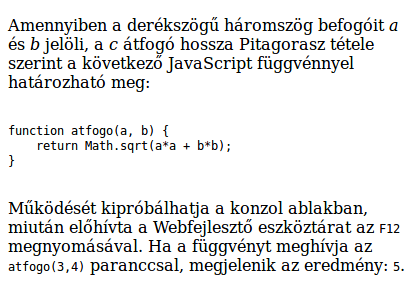
\includegraphics[width=\textwidth]{kod.png}
  \end{columns} 
\end{frame}

%80
\begin{frame}
  \begin{exampleblock}{\textattachfile{kod.html}{kod.html}}
    \scriptsize
    \lstinputlisting[style=HTML,linerange={8-20},numbers=left,firstnumber=8]{kod.html}
  \end{exampleblock}
\end{frame}

%81
\begin{frame}
  \begin{columns}[c]
    \column{0.6\textwidth}
      Induljon ki a \textattachfile{vizsga.txt}{vizsga.txt} fájlból, 
      és készítse el ebből azt a HTML fájlt, ami a mellékelt 
      ábrának megfelelően jelöli
      \begin{itemize}
        \item a program változóinak nevét,
        \item a függvény kódját,
        \item a lista (lehetséges válaszok) elemeit!
      \end{itemize}
    \column{0.35\textwidth}
      \begin{exampleblock}{\textattachfile{vizsga.html}{vizsga.html}}
        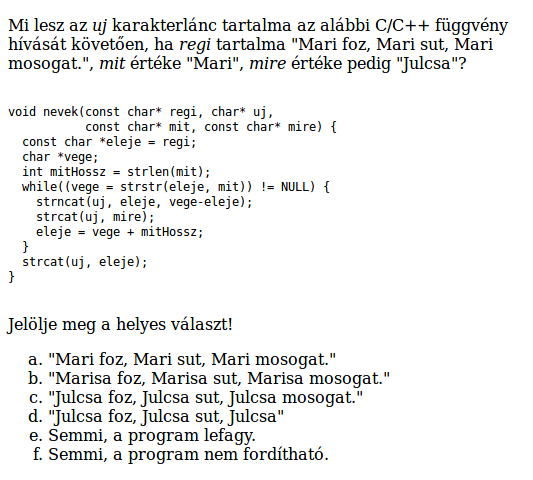
\includegraphics[width=\textwidth]{vizsga.png}
      \end{exampleblock}
  \end{columns} 
\end{frame}
